\documentclass[sigplan,screen,natbib=false]{acmart}

\usepackage{blindtext}
\usepackage{amsmath}
%\usepackage{amssymb}
\usepackage{graphicx}
\usepackage{biblatex}
\usepackage{tikz}
\usepackage{algorithm}
\usepackage{algpseudocode}

\graphicspath{ {./} }
\addbibresource{bibliography.bib}

%\usetikzlibrary{positioning}
%\usetikzlibrary{shapes}

%\newcommand{\vct}[1]{\boldsymbol{#1}}
%\newcommand{\relu}{\mathit{ReLU}}
%\newlength{\vnd}
%\newlength{\hnd}
%\newlength{\vds}
%\newcommand{\scl}{1}
%\tikzset{>=stealth}

%% Use the following for comments
\newcommand{\dmcmt}[1]{\textcolor{blue}{#1}}
\newcommand{\kmcmt}[1]{\textcolor{red}{#1}}
\newcommand{\sncmt}[1]{\textcolor{green}{#1}}
\newcommand{\todo}[1]{\textcolor{orange}{TODO: #1}}

%% Common stuff like ReLU
% TODO refactor to use this
\newcommand{\relu}{\textit{ReLU}}
\newcommand{\cnc}{$\mathcal{N}$}
\newcommand{\abs}{$\mathcal{N'}$}
\newcommand{\abcrown}{$\alpha\beta-CROWN$ \todo{cite}}
\newcommand{\acasxu}{ACAS Xu \todo{cite}}
\newcommand{\mnist}{VNNComp MNIST \todo{cite}}
\newcommand{\pgd}{PGD-attack \todo{cite}}
\newcommand{\cegar}{CEGAR \todo{cite}}
\newcommand{\dnn}{DNN}

\title{Title}
\author{Sanaa Siddiqui, Diganta Mukhopadhyay, Afzal Mohammed, Hrishikesh
Karmarkar, Kumar Madhukar }

\begin{document}

\maketitle
\todo{ Add affiliations}

Neural Networks are increasingly being used in several safety critical
applications, including medical imaging, self driving cars and aircraft
collision detection. To gain trust on the networks being deployed in safety
critical domains and reduce the risk of safety violations, several techniques
based on formal analysis has been proposed, including formal verification and
formal explainability. However, the scalability of these techniques is highly
sensitive to the size of the networks involved, limiting the applicability of
these techniques to real-world networks. To handle these scalability issues,
structural abstraction based on syntactic techniques have been proposed, and
while these provide formal soundness guarantees, they do not take into account
the semantic behavior of the network. On the other hand, neural network
compression and semantic abstraction \dmcmt{Jan, few lines in intro}
techniques take into account this information, but the soundness guarantees they
provide are generally much weaker, if at all present. We propose to combine both
the semantic and syntactic approaches into a single framework to try to obtain
the best of both worlds, guiding our abstraction using global semantic
information while still providing concrete soundness guarantees based on
syntactic constraints. We do this by constructing a partial order of best
possible merges using global semantic information, and represent it using a
tree-like data structure. Then we follow this tree to perform syntactic merge
and example guided \sncmt{Some other wording?} refinement operations. This
allows us to obtain abstract networks that is guided by global semantic
information while providing concrete soundness guarantees. We demonstrate the
effectiveness of these abstractions on standard neural network benchmarks via
experiments.

    
\section{Introduction}

\todo{ Re-work wrt new experiments section }

Advances in Deep Neural Networks (DNNs) have enabled the scalable solution
of several previously intractable problems like image recognition.\todo{
cite} Due to this, DNNs have been increasingly assumed a central role across
various domains. These include several safety critical domains like healthcare
\cite{b1},
where they contribute significantly to medical diagnostics and predictive
analysis \cite{b2}, and autonomous vehicles, where DNNs serve as the
backbone for sophisticated perception systems, supporting tasks such as object
recognition and decision-making \cite{b3}. 

%\hide{However, it is crucial to acknowledge
%that these applications operate in safety-critical settings, necessitating DNNs
%to exhibit correct and accurate behavior.}

However, DNNs are well known to be vulnerable to adversarial attacks \todo{
cite} and can produce unexpected behaviours which in safety critical domains can
lead to unsafe situations. Therefore, there is a critical need to guarantee the
precise functionality and safety of these DNNs that are deployed in
safety-critical environments, to build trust on the systems that utilize these
DNNs.

A number of verification techniques have been proposed to validate
the reliability of DNNs in safety-critical settings \cite{b4, b5}, including
those based on abstract interpretation, branch and bound, etc. \todo{ cite
} However, since DNN verification is NP-Hard \todo{ cite}, verification
techniques for DNNs often face scalability issues. Our work is based on
counterexample guided abstraction refinement \cite{cegar-nn} and aims to
alleviate this issue by reducing the verification problem for a large
\textit{concrete} DNN \cnc into an over-approximate query involving a smaller
\textit{abstract} DNN \abs. This is done by \textit{merging} groups of neurons
belonging to the same \textit{merge group} in \cnc into single neurons in \abs.
\todo{ appeal to later sections via ref.}
Then, this smaller query may be dispatched using any existing technique, thus
extending the scalability of that technique. 

While counterexample guided abstraction refinement based on structural
abstraction has been proposed \cite{cegar-nn} \todo{ cite others}, in
several cases these techniques are forced to refine all the way to the original
network, resulting in a query that is as complicated as the original
verification problem we started with. We posit that this is because the
refinement process does not
identify which merges should be prioritised based on the semantics of the
network, instead removing a single node from a merge group, leaving potentially
equally over-approximate merges in the network. This leads to situations where,
after several refinement steps, \abs has a large number of singleton merge
groups, leading to a large yet over-approximate abstract network. 
\todo{ refer to later sections with eg demoing this.} 

In this work we utilise measures of similarities between neurons explored in
\todo{ cite, check Jan Kretinsky's and others works} to build a partial
order of possible merges in each layer capturing the priority each merge should
get during the refinement process. This allows us to use the information from a
spurious counterexample to cut a merge group in a manner that eliminates the
merge operation that has been estimated to contribute most to the
over-approximation. This avoids the proliferation of singleton merge groups in
\abs, and leads to a smaller and a tighter abstraction.

We describe a way to efficiently implement this partial order based refinement
procedure to be able to iterate through potential refinements with minimal
computational overheads. We do this by creating tree-based data structures that
allows us to pre-compute a significant portion of the relevant information at
the beginning of the refinement loop. Then, refinement operations can be
performed via very quick index manipulations. This allows us to iterate through
and screen several possible refinements fast before committing to a solver call.


\section{Background}

\dmcmt{ 
    An example of Elboher's Refinement where we get a lot of singletons
}
\section{Background}
\subsection{Neural Network}

\dmcmt{There was some general definitions of what an nn is in this section,
removed for now, nor really necessary, maybe can add a notation section if at
all necessary}

\sncmt{Notation is important. Will be required in the upcoming sections.}

We conceptualize neural networks as directed acyclic graphs 
comprising three types of layers: the input layer, intermediate hidden layers, 
and the output layer. Our goal is to focus on the abstracting feed forward networks, 
where neuron values are computed based on preceding layer neuron values. 
Neurons in our network are denoted as $n_{(i,j)}$, where `$i$' signifies the 
neuron number in layer `$j$'. The weight matrix between layers `${j-1}$' and `$j$' 
is denoted as `$W_{{j-1}, j}$', and the bias matrix for layer `$i$' is denoted as 
`$B_{i}$'. The value of the `$i^{th}$' neuron in layer `$j$' for a given input vector 
is represented by `$v_{(i,j)}$', and `$V_{j}$' encompasses all such `$v_{(i,j)}$' values for layer 
`$j$'. The function $o_{(i, j)}$ takes a list of input vectors and outputs a list of
corresponding `$v_{(i,j)}$' for a particular neuron $n_{(i, j)}$. 

The computation of `$V_{j}$' involves applying an ``activation function ($\phi$)" 
to the ``weighted sum":

\[V_{j} = \phi(W_{{j-1}, j} \cdot V_{j-1} + B_{j}).\] 

We confine our activation function to the Rectified Linear Unit (ReLU), 
which can be expressed as $V_{j} = \max(W_{j-1, j} \cdot V_{j-1} + B_{j}, 0)$.

\subsection{ Formal Analysis of Neural Networks }
\label{s:form-an}
\dmcmt{This section used to be titled Neural Network Verification, and explained
    the general idea of neural net verif, and some stuff on prop encoding. We
    are not doing exclusively verif. So, some more general and shorter
    discussion on formal analysis of nn added.}

Several techniques and methods have been studied to improve the reliability and
trustworthiness of \dnn deployed in safety critical settings via formal
analysis. This includes verifying \dnn with respect to a given
safety property \cite{reluplex, cegar-nn, deeppoly, cegarette, cleverest-nn,
conv-abs-gk, deep-abstract, lin-comb-abs-jan}, providing formal explanations of
the behavior of the \dnn \cite{minimal-image-fxai, overview-fxai}, and others.
\dmcmt{Is the and others okay? Ref the backdoor attacks work?} To provide the
formal guarantees behind the analysis performed, all of these techniques rely on
making \textit{neural network queries}. 

These neural network queries are of the form $(P, \mcnc, Q)$, and ask if
for all inputs $x$ to $\mcnc$ for which the formula $P$ holds
the formula $Q$ also holds on the output $\mcnc(x)$. While there are several
tools that can handle such queries, like \marabou and \abcrown, scalability
remains an issue, and so reducing the size of \cnc is desirable.

\subsection{Semantic Compressions and Abstractions with Empirical Guarantees}
\label{s:emp-abs}
\dmcmt{What is a better word than 'weak' here? Does 'empirical' work here?}

Several techniques utilise semantic information, typically extracted via
simulation of the \dnn, to obtain \abs. \dmcmt{Say: to improve scalability? }.
Neural network compression techniques \todo{cite}, produce small \abs, but the
behavior of \abs in connection to \cnc is only characterized empirically.
Similarly, some semantic abstraction techniques \cite{lin-comb-abs-jan} provide
bi-simulation guarantees bounding the difference in the behavior of \abs and
\cnc on a finite set of input points, typically a subset of the training
dataset. Since these techniques characterize the behavior of \abs only on a
finite set of
input points, the trust obtained on the connection between \cnc and \abs is only
of a empirical nature.
Other techniques like \cite{deep-abstract} use bi-simulation to lift
interval bound propagation performed on \abs to get sound bounds on \cnc. While
this does provide a sound proof, interval bounds are typically not strong enough
to prove many interesting and practically relevant neural network queries.
\todo{cite}

\subsection{Concrete Guarantees on Neural Network Abstractions}
\label{s:conc-abs}
\kmcmt{We need to add one is good for analysis and one is good for proofs.
Not in negative light.} \dmcmt{ Even for analysis, we are trying to claim that
our concrete guarantees are better than the empirical ones right? We show a case
of proof, and a case of compression, so things are clear right?}

The notion of providing concrete guarantees on the behavior of \abs relative to
\cnc has been formalized in \cite{cegar-nn}. In particular, guarantees of the
form $\forall x, \mabs(x) \geq \mcnc(x)$ \dmcmt{
Should I format this as definition?} are useful as a general notion of concrete
guarantees in many settings. Two such settings are as follows: 

Firstly, since any general neural network query can be converted to a query of
the form $(P, \mcnc, y < c)$ for some $c$ \cite{cegar-nn, reluplex} \todo{See
\cite{cegar-nn}, they have another citation for this encoding} \dmcmt{It seems
that \cite{cegar-nn}, \cite{reluplex} and we have 3 different encodings, but
generally based on the same idea of implementing bool combs via extra nn
layers}, such a guarantee is
useful for dispatching the query on a smaller network \cite{cegar-nn, cegarette,
cleverest-nn}. This immediately makes an \abs with these guarantees useful for
accelerating several formal analysis techniques (Section \ref{s:form-an}).

Furthermore, such guarantees are also useful for safe compression of \dnn.
Consider the case of medical diagnosis\todo{cite} or aircraft
collisions\cite{acasxu}, where
for safety reasons, a classifier should be biased towards not producing false
negatives. Guarantees such as above can formally ensure that the compressed \abs
never produces any more false negatives than \cnc. \todo{Ref next sections}.
\dmcmt{Should this be here?}

Therefore, in this work we focus on developing a framework\dmcmt{Is this word
here okay?} that produces
abstract networks with this guarantee.

\subsection{Quality of Abstractions and Spurious Points}
\label{s:qual}

A generally useful notion with respect to abstraction is \textit{quality},
which we as the number of \textit{spurious inputs} that witness a difference in
the relevant behavior of \abs and \cnc. In the context of using \abs to
accelerate formal analysis of \dnn, these spurious inputs may simply be
\textit{spurious counterexamples} \cite{cegar-nn, cleverst-nn} to a query
involving \abs that are not counterexamples for the same query involving \cnc.
This notion may be generalized to other uses of abstractions as well. For
instance, for safe compressions, they may be inputs from a dataset which
are falsely classified as positive by \abs. \todo{Ref section}

\subsection{Syntactic Neural Network Splitting and Merging}
\label{s:nn-sam}

\dmcmt{Given that this section is critical to understanding our soundness
    guarantees, and that this is mostly existing work, how much space should be
spent here? Can we trust reader to read \cite{cegar-nn}}

\dmcmt{Start a running example here}

To transform \cnc into \abs so that the soundness guarantees hold, we follow
\cite{cegar-nn} to \textit{split} neurons in \cnc into copies labelled with
labels from \{\inc, \dec\} $\times$ \{\posc, \negc\} so that any
increase (decrease) in the value of a neuron labelled
\inc (\dec) only leads to an increase in output value. Then,
following \cite{cegar-nn}, a sound abstraction can be obtained by
\textit{merging} all similarly labelled neurons as follows: if the neurons have
the label \inc (\dec), replace incoming edges from the same
previous layer neuron with a single edge with the maximum (minimum) of the
original edge weights. Outgoing edges to the same next layer neuron are replaced
with a single edge with the sum of the weights for both the \inc and \dec case.

\dmcmt{Do we need to add a reference for 2-class? It may help shorten section.} 

We make a slight modification to the above: as a first optimization step, we
re-merge the two copies of the \abs neurons that are otherwise the same, but
have \posc and \negc labels respectively. This can always be done without
changing the behavior of the network since these copies will have the same \inc,
\dec labels and the same incoming weights. \dmcmt{Is this clear? Is it better to
write this as a lemma, and then put a proof in appendix?} This optimisation
allows us to discard the \posc and \negc class information, and reduces the size
of the maximally merged network.

Note that this process only considers the syntactic structure of the network, no
semantic information is used.

\subsection{ Syntactic Refinement }
\dmcmt{Jan Kretinsky's abstraction is based on semantic info, refinement is not.
Given this, do we really need to talk about Jan's refinement here? If yes,
how to weave it in?}

The fully merged network obtained in Section \ref{s:nn-sam} may not have
sufficient quality (Section \ref{s:qual}) to be useful. For instance, when doing
formal analysis, there may be too many spurious counterexamples. In such
situations, a common approach to obtain a better quality \abs is to perform
refinement steps based on a spurious counterexample $x$ \cite{cegar-nn,
cegarette, cleverest-nn}. \dmcmt{While \cite{cegar-nn} does it only for spurious cexes,
it can be directly extended to spurious inputs. But, I'm speaking in terms of
sp cex here to avoid confusion. Should I say spurious input instead?} In
existing techniques this is typically done restoring a single neuron in \cnc
that had been merged \abs. The neuron chosen is typically one whose contribution
to $x$ is estimated to be the highest.

These techniques, however, do not consider any semantic behavior to guide their
refinement. As such, the refinement process tends to produce a large number of
restored neurons identical to neurons in \cnc, leading to and \abs of large
size, while retaining a single abstract neuron formed by merging a large group
of neurons in \cnc, affecting the quality of \abs.  \todo{example}

\begin{figure}[htbp]
    \centering
    \begin{tikzpicture}[scale=0.5] % Adjust the scale factor as needed
      % Your TikZ code goes here
      \draw (5,-5) circle (1cm);
      \node at (5,-5) {$n_{(1,3,+)}$};
      \draw (5,-2) circle (1cm);
      \node at (5,-2) {$n_{(1,2,+)}$};
      \draw (0,2) circle (1cm);
      \node at (0,2) {$n_{(0,0)}$};
      \node at (-2,2) {[-1, 1]};
      \draw (0,-2) circle (1cm);
      \node at (-2,-2) {[-1, 1]};
      \node at (0,-2) {$n_{(0,1)}$};
      \draw (10,0) circle (1cm);
      \node at (10,0) {$n_{(2,0)}$};
      \node at (12,0) {$< 6.1$};
      \draw (5, 5) circle (1cm);
      \node at (5,5) {$n_{(1,0,+)}$};
      \draw (5, 2) circle (1cm);
      \node at (5,2) {$n_{(1,1,+)}$};

    \draw (1, -2) -- (4, -5);
    \node at (3.25,-4.75) {0.5};
    \draw (1, 2) -- (4, -5);
    \node at (4,-4) {1};
    \draw (1, -2) -- (4, -2);
    \node at (3.45,-2.5) {0.55};
    \draw (1, 2) -- (4, -2);
    \node at (4.25,-0.75) {0.95};
    \draw (1, -2) -- (4, 2);
    \node at (4.25, 0.75) {0.95};
    \draw (1, -2) -- (4, 5);
    \node at (4, 4) {1};
    \draw[solid, postaction={decorate, decoration={text along path,
          text={0.55}, text align=right, raise=1mm}}] (1, 2) -- (4, 2);
    \draw[solid, postaction={decorate, decoration={text along path,
          text={0.5}, text align=right, raise=1mm}}] (1, 2) -- (4, 5);

    \draw[solid, postaction={decorate, decoration={text along path,
        text={1}, text align=center, raise=1mm}}] (6,-5) -- (9, 0);
    \draw[solid, postaction={decorate, decoration={text along path,
        text={1}, text align=center, raise=1mm}}] (6,-2) -- (9, 0);
    \draw[solid, postaction={decorate, decoration={text along path,
        text={1}, text align=center, raise=1mm}}] (6,2) -- (9, 0);
    \draw[solid, postaction={decorate, decoration={text along path,
        text={1}, text align=center, raise=1mm}}]  (6, 5) -- (9, 0);
      
    \end{tikzpicture}
    \caption{Original Network and Property}
    \label{fig:Original_Net_Property}
  \end{figure}
  

\begin{figure}[htbp]
    \centering
    \begin{tikzpicture}[scale=0.5] % Adjust the scale factor as needed
      % Your TikZ code goes here
      \draw[line width=1pt, fill=orange!30] (5,0) circle (1cm);
      \node at (5,0) {$a_1$};
      \node [text=red] at (5,1.5) {\textbf{1.55}};
      \draw[line width=1pt, fill=blue!30] (0,2) circle (1cm);
      \node at (0,2) {$n_{(0,0)}$};
      \node [text=red] at (-2,2) {\textbf{0.55}};
      \draw[line width=1pt, fill=blue!30] (0,-2) circle (1cm);
      \node [text=red] at (-1.5,-2) {\textbf{1}};
      \node at (0,-2) {$n_{(1,0)}$};
      \draw[line width=1pt, fill=green!30] (10,0) circle (1cm);
      \node at (10,0) {$n_{(0,2)}$};
      \node [text=red] at (12,0) {\textbf{6.2}};
    \draw[myarrow] (1, -2) to (4, 0);
    \node at (2.5,-1.25) {1};
    \draw[myarrow] (1, 2) to (4, 0);
    \node at (2.5,1.25) {1};


    \draw[->,  >=angle 45, thick, postaction={decorate, decoration={text along path,
        text={4}, text align=center, raise=1mm}}] (6,0) -- (9, 0);
    % \draw[solid, postaction={decorate, decoration={text along path,
    %     text={1}, text align=center, raise=1mm}}] (6,-2) -- (9, 0);
    % \draw[solid, postaction={decorate, decoration={text along path,
    %     text={1}, text align=center, raise=1mm}}] (6,2) -- (9, 0);
    % \draw[solid, postaction={decorate, decoration={text along path,
    %     text={1}, text align=center, raise=1mm}}]  (6, 5) -- (9, 0);
      
    \end{tikzpicture}
    \caption{Fully Abstracted Network}
    \label{fig:full_abstract_net}
  \end{figure}
  

\begin{figure}[htbp]
    \centering
    \begin{tikzpicture}[scale=0.5] % Adjust the scale factor as needed
      % Your TikZ code goes here
      \draw[line width=1pt, fill=orange!30] (5,2) circle (1cm);
      \node at (5,2) {$a_2$};
      \node [text=red] at (5,0.75) {1.7};
      \draw[line width=1pt, fill=pink!30] (5,-2) circle (1cm);
      \node at (5,-2) {$n_{(3,1)}$};
      \node [text=red] at (5,-3.5) {1.375};
      \draw[line width=1pt, fill=blue!30] (0,2) circle (1cm);
      \node at (0,2) {$n_{(0,0)}$};
      \node [text=red] at (-2,2) {1};
      \draw[line width=1pt, fill=blue!30] (0,-2) circle (1cm);
      \node [text=red] at (-1.75,-2) {0.75};
      \node at (0,-2) {$n_{(1,0)}$};
      \draw[line width=1pt, fill=green!30] (10,0) circle (1cm);
      \node at (10,0) {$n_{(0,2)}$};
      \node [text=red] at (12,0) {$6.475$};
    \draw[->, >= angle 45, thick, postaction={decorate, decoration={text along path,
    text={0.5}, text align=center, raise=1mm}}](1, -2) -- (4, -2);
   
    \draw[myarrow] (1, -2) -- (4, 2);
    \node at (3.75,1.25) {1};
  
    \draw[myarrow] (1, 2) -- (4, -2);
    \node at (3.75,-1.25) {1};
  
    \draw[->, >= angle 45, thick, postaction={decorate, decoration={text along path,
    text={0.95}, text align=center, raise=1mm}}] (1, 2) -- (4, 2);
   


    \draw[->, >= angle 45, thick, postaction={decorate, decoration={text along path,
    text={1}, text align=center, raise=1mm}}] (6,-2) -- (9, 0);
    \draw[->, >= angle 45, thick, postaction={decorate, decoration={text along path,
    text={3}, text align=center, raise=1mm}}] (6, 2) -- (9, 0);

    \end{tikzpicture}
    \caption{Refine Step 1: Culprit Neuron is 3}
    \label{fig:refine_step_1}
  \end{figure}
  

\begin{figure}[htbp]
    \centering
    \begin{tikzpicture}[scale=0.5] % Adjust the scale factor as needed
      % Your TikZ code goes here
      \draw (0,2) circle (1cm);
      \node at (0,2) {$n_{(0,0)}$};
      \node [text=red] at (-2,2) {1};
      \draw (0,-2) circle (1cm);
      \node [text=red] at (-2,-2) {1};
      \node at (0,-2) {$n_{(1,0)}$};
      \draw (5,4) circle (1cm);
      \node at (5,4) {$n_{(0,1)}$};
      \node [text=red] at (5,2.5) {1.5};
      \draw (5,-4) circle (1cm);
      \node at (5,-4) {$n_{(3,1)}$};
      \node [text=red] at (5,-5.5) {1.5};
      \draw (5,0) circle (1cm);
      \node at (5,0) {$a_3$};
      \node [text=red] at (5,-1.5) {1.9};
      \draw (10,0) circle (1cm);
      \node at (10,0) {$n_{(0,2)}$};
      \node [text=red] at (12,0) {$6.8$};
    \draw[->, >= angle 45, postaction={decorate, decoration={text along path, 
    text={0.5}, text align=center, raise=1mm}}](1, 2) -- (4, 4);
    \draw[myarrow](1, -2) -- (4, 4);
    \node at (3.75,3) {1};
    \draw[myarrow](1, 2) -- (4, 0);
    \node at (3.75,1) {0.95};
    \draw[myarrow](1, -2) -- (4, 0);
    \node at (3.75,-1) {0.95};
    \draw[myarrow](1, 2) -- (4, -4);
    \node at (3.75,-3) {1};
    \draw[->, >= angle 45, postaction={decorate, decoration={text along path, 
    text={0.5}, text align=center, raise=1mm}}](1, -2) -- (4, -4);
    \draw[->, >= angle 45, postaction={decorate, decoration={text along path,
    text={1}, text align=center, raise=1mm}}] (6,-4) -- (9, 0);
    \draw[-> , >= angle 45 , postaction={decorate, decoration={text along path,
    text={2}, text align=center, raise=1mm}}] (6,0) -- (9, 0);
    \draw[->, >= angle 45, postaction={decorate, decoration={text along path,
    text={1}, text align=center, raise=1mm}}] (6,4) -- (9, 0);
   
    % \draw (1, -2) -- (4, 2);
    % \node at (3.75,1.25) {1};
  
    % \draw (1, 2) -- (4, -2);
    % \node at (3.75,-1.25) {1};
  
    % \draw[solid, postaction={decorate, decoration={text along path,
    % text={0.95}, text align=center, raise=1mm}}] (1, 2) -- (4, 2);
   


    % \draw[solid, postaction={decorate, decoration={text along path,
    % text={1}, text align=center, raise=1mm}}] (6,-2) -- (9, 0);
    % \draw[solid, postaction={decorate, decoration={text along path,
    % text={3}, text align=center, raise=1mm}}] (6, 2) -- (9, 0);

    \end{tikzpicture}
    \caption{Refine Step 2: Culprit Neuron is 0}
    \label{fig:refine_step_2}
  \end{figure}
  



\section{Our Method}

\dmcmt{
    In same example, we immediately arrive at a better picture. 
    This picture is equivalent to refining and merging back in the Elboher's
    setting.
} 
\section{Methodology}
\label{s:semantic-closeness}

In this work we aim to utilize information from the semantic behavior of \cnc to
better control and guide the refinement process producing higher quality \abs
while retaining concrete soundness. 

In particular, we define a \textit{semantic
closeness metric} that captures how close the semantic-behavior of two 
neurons are (Section \ref{s:semantic-closeness}). We utilise this semantic
closeness metric to arrange the merge
operations into a tree where lower quality merges involving semantically far
neurons appear higher and can be refined with higher priority (Section
\ref{s:tree}). 

Using this tree we build a framework where refinement can
be done by making cuts of this tree, while still providing concrete soundness
guarantees (Section \ref{s:refinement}). We show that
the merges retained in this refinement process is optimal with respect to the
semantic information (Section \ref{s:optimal-tree}).
This allows us to avoid restoring large number of single neurons(see Section
\ref{s:nn-sam}) and lets us retain merge operations of higher quality. Thus, we
produce an \abs of the desired quality with a much smaller size. 

%While the choice of which nodes to leave merged together is guided by the cuts
%of the tree, the weights attached to the abstract nodes are still chosen
%by following the procedures from Section \ref{s:nn-sam} and \cite{cegar-nn}.
%Thus, the concrete soundness guarantees still hold for the \abs obtained.
%\dmcmt{This point is repeated in \ref{s:refinement}, but this should be okay
%right?}

%In the following sections we describe a general framework for such a unified
%syntactic and semantic refinement process, describing each component in detail.

Using these components, we propose a general abstraction-refinement loop based
framework (Section \ref{s:abs-ref-fw}) that combines syntactic merge operation
with semantic behavior. This framework is able to utilise \gencex from any
source and continually refine until a \abs of desired quality is achieved.

\subsection{Semantic Closeness Factor}
\label{s:semantic-closeness}

\todo{If we are able to get the characterestic based exps run, we can talk
    about that as well.
}

To guide the semantic abstraction process, we define a \textit{semantic
closeness metric} $\cls$: $\cls(\nr{i_1}{l}, \nr{i_2}{l})$ is function that
takes two neurons $\nr{i_1}{l}$ and $\nr{i_2}{l}$ in
the same layer $l$, and returns a real number that
captures how close the behaviors of $\nr{i_1}{l}$ and $\nr{i_2}{l}$ are from a
semantic point of view. The number returned by $\cls$ should be smaller for
neurons whose semantic behavior is closer. Intuitively, this metric would
characterise the semantic behavior of the
neurons in layer $l$ relative to each other, and prioritise certain merges over
others. 

Depending on the application, the precise definition of this metric may be
chosen in various ways. We note that our framework is agnostic to the particular
choice of semantic metric, and a concrete soundness guarantee holds for any such
choice. Inspired by \cite{deep-abstract}, in we chose as the
semantic closeness metric how close the functions computed by the two neurons
are: $||\nrf{i_1}{l} - \nrf{i_2}{l}||$. 

However, since $\nrf{i_1}{l}$ and $\nrf{i_2}{l}$ are functions, computing
$||\nrf{i_1}{l} - \nrf{i_2}{l}||$ precisely is not feasible.
Therefore, we estimate it using a sample set of inputs $X$: $||\ob{i_1}{l}($X$)
- \ob{i_2}{l}($X$)||_2$. This $X$ may be chosen in many ways, for example, it
may be a set of randomly chosen input values satisfying $P$ when
abstracting with respect to a query $(P, \mcnc, Q)$
(Section \ref{s:exp-mnist-rob}), or a dataset when attempting to find a
safe compression (Section \ref{s:exp-mnist-comp}).

\subsection{Tree of Merges}
\label{s:tree}

We use $\cls$ to create a tree structure to prioritise merges wherein leaf nodes
represent the original neurons, and 
non-leaf nodes represent merge operations. The construction of the tree 
follows a bottom-up approach, starting from individual neurons, 
greedily performing the merge operation involving the most similar groups of
neurons, and delaying the merging of dissimilar ones. The resulting tree
captures an optimal ordering of merge operations (Section \ref{s:optimal-tree}).

Note that $\cls$ only provides us
with a similarity measure for pairs of neurons. For this tree construction
algorithm to work we must extend this to a semantic closeness
metric between groups of neurons
$\{\nr{i_1}{l}, {\cdots}, \nr{i_p}{l}\}$ and $\{\nr{j_1}{l}, {\cdots},
\nr{j_q}{l}\}$. To do this we take the pairwise maximum since it captures the
notion of the largest difference in semantic behavior and ensures that the tree
is optimal (Section \ref{s:optimal-tree}): 

\begin{equation*}
\begin{aligned}
    \max_{k_1 \in \{1, {\cdots}, p\},
    k_2 \in \{1, {\cdots}, q\}} \cls( \nr{i_{k_1}}{l}, \nr{j_{k_2}}{l} )
\end{aligned}
\end{equation*}

\dmcmt{Is the above notation necessary, or can we just say pairwise maximum and
refer to algo?}

This process is detailed in Algorithm \ref{a:build-tree}.

\begin{algorithm}
\caption{Building the Tree}
\label{a:build-tree}
\begin{algorithmic}[1]

    \Require Neurons $\{\nr{i_1}{l}, {\cdots}, \nr{i_r}{l}\}$ with same class,
    Closeness metric $\cls$

    
    \State Initialize a Binary Tree $T$ with leaves as
        $\{m_1, {\cdots}, m_r\}$ corresponding to $\{ \nr{i_1}{l}, {\cdots},
        \nr{i_r}{l} \}$
    %\State Initialize map $M(m_k) = \{ \nr{i_k}{l} \}$ taking tree nodes to sets
    %    of neurons in corresponding merge group
    \State Initialize $Q=\{m_1, {\cdots}, m_r\}$ as the set of leaf nodes.

    \Function{PairwiseMax}{$m, m'$}
        
            \State Let $L, L'$ be leaves of sub-tree rooted at $m, m'$

            \Return $\max_{\nr{i_{k}}{l} \in S, \nr{i_{k'}}{l} \in S'} 
                \cls( \nr{i_{k}}{l}, \nr{i_{k'}}{l} )$

    \EndFunction

    \While{$|Q|>1$}
        \State $m_{j_1}, m_{j_2} = \arg\min_{\substack{m, m' \in Q}} 
            \text{PairwiseMax}(m, m')$
        \State Add new node $m_{j_3}$ to $T$ 
        \State Make $m_{j_1}, m_{j_2}$ children on $m_{j_3}$
        \State Remove $m_{j_1}, m_{j_2}$ from $Q$ and add $m_{j_3}$ to $Q$.
    \EndWhile

    \Ensure Tree of merges $T$
\end{algorithmic}
\end{algorithm}

For instance, considering the middle layer in Figure
\ref{fig:Original_Net_Property}, $\nr{0}{1}$ and $\nr{1}{1}$ are semantically
closest. Thus, in the tree, we merge these two first to get the node $m_4$.
Then, the two semantically closest pairs are given by $\nr{2}{1}$ and
$\nr{3}{1}$, so they are merged to $m_5$. Finally, $m_4$ and $m_5$ gets merged
to $m_6$. This gives us the tree seen in the top half of Figure
\ref{fig:Order_of_merging}.

As we progress up the tree, the maximum value of $\cls$ between any two neurons
involved in a merge increases. Thus, as we move up the tree, the imprecision
introduced by the merge operation increases. 

In our example, the merge operation
$m_4$ involves $\{\nr{0}{1}, \nr{1}{1}\}$, while $m_6$ involves $\{\nr{0}{1},
\nr{1}{1}, \nr{2}{1}, \nr{3}{1}\}$. Since the semantic behavior of $\nr{0}{1}$
and $\nr{1}{1}$ are closer than $\nr{0}{1}$, $\nr{1}{1}$, $\nr{2}{1}$,
$\nr{3}{1}$, operation $m_4$ represents a less coarse abstraction than $m_6$.

For our choice of $\cls$, (Section \ref{s:semantic-closeness}), Algorithm
\ref{a:build-tree} reduces to \hcluster, allowing us to leverage existing
efficient implementations \cite{scipy-hcluster-linkage}. Nonetheless, the
general algorithm presented here will work for any choice of $\cls$.

\subsection{Tree-cuts and Refinement}
\label{s:refinement}



\begin{figure}[htbp]
    \centering
    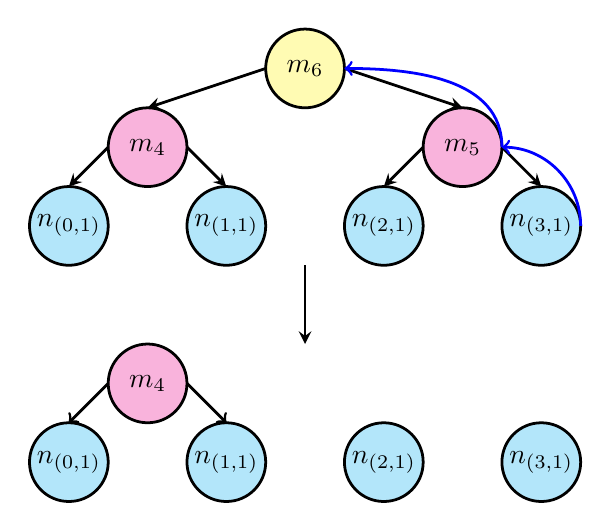
\begin{tikzpicture}[scale=0.5] % Adjust the scale factor as needed
        % Your TikZ code goes here
        \draw[line width=1pt,fill=yellow!30] (0,0) circle (1cm);
        \node at (0,0) {$m_6$};
        \draw[line width=1pt, fill=magenta!30] (-4,-2) circle (1cm);
        \node at (-4,-2) {$m_4$};
        \draw[line width=1pt, fill=magenta!30] (4,-2) circle (1cm);
        \node at (4,-2) {$m_5$};
        \draw[line width=1pt, fill=cyan!30] (-6,-4) circle (1cm);
        \node at (-6,-4) {$n_{(0,1)}$};
        \draw[line width=1pt, fill=cyan!30] (-2,-4) circle (1cm);
        \node at (-2,-4) {$n_{(1,1)}$};
        \draw[line width=1pt, fill=cyan!30] (6,-4) circle (1cm);
        \node at (6,-4) {$n_{(3,1)}$};
        \draw[line width=1pt, fill=cyan!30] (2,-4) circle (1cm);
        \node at (2,-4) {$n_{(2,1)}$};
        \draw[-> , >=stealth,line width=1pt] ({0 + cos(180)},{0 + sin(180)}) -- (-4,-1);
        \draw[->, >=stealth, line width=1pt] ({0 + cos(0)},{0 + sin(0)}) -- (4,-1);
        \draw[->, >=stealth, line width=1pt] ({-4 + cos(180)},{-2 + sin(180)}) -- (-6,-3);
        \draw[->, >=stealth, line width=1pt] ({-4 + cos(0)},{-2 + sin(0)}) -- (-2,-3);
        \draw[->, >=stealth, line width=1pt] ({4 + cos(180)},{-2 + sin(180)}) -- (2,-3);
        \draw[->, >=stealth, line width=1pt] ({4 + cos(0)},{-2 + sin(0)}) -- (6,-3);
        
        % Curved arrow
        \draw[->, color=blue, line width=1pt] (7, -4) to[out=90, in=0] (5, -2);
        \draw[->, color=blue, line width=1pt] (5, -2) to[out=90, in=0] (1, 0);
        \draw[->, >=stealth, line width=1pt] (0,-5) to (0,-7);

        \draw[line width=1pt, fill=magenta!30] (-4,-8) circle (1cm);
        \node at (-4,-8) {$m_4$};
        \draw[line width=1pt, fill=cyan!30] (-6,-10) circle (1cm);
        \node at (-6,-10) {$n_{(0,1)}$};
        \draw[line width=1pt, fill=cyan!30] (-2,-10) circle (1cm);
        \node at (-2,-10) {$n_{(1,1)}$};
        \draw[line width=1pt, fill=cyan!30] (6,-10) circle (1cm);
        \node at (6,-10) {$n_{(3,1)}$};
        \draw[line width=1pt, fill=cyan!30] (2,-10) circle (1cm);
        \node at (2,-10) {$n_{(2,1)}$};
    
        \draw[->, line width=1pt] ({-4 + cos(180)},{-8 + sin(180)}) -- (-6,-9);
        \draw[->, line width=1pt] ({-4 + cos(0)},{-8 + sin(0)}) -- (-2,-9);

    \end{tikzpicture}
    \caption{Trees and Cuts}
    \label{fig:Order_of_merging}
\end{figure}


In our abstraction refinement loop, we start with the fully merged network.
Then, whenever we get a \gencex $\vct{\beta}$ (Section \ref{s:qual}), we wish to
refine the network, that is, we wish to chose which
neurons should remain merged. Intuitively, this choice should be guided
two factors: optimising with respect to the semantic behavior of the network,
and attempting to eliminate $\vct{\beta}$.

The tree produced in the previous Section \ref{s:tree} captures the semantic
behavior, and we use it to guide the refinement process as follows:
Any cut of the tree produces a set of trees. Then,  
the groups of neurons that we chose to keep merged correspond to the leaf nodes
of the  these trees. Therefore finding a refinement is reduces to finding a cuts
in the tree.

To attempt to eliminate $\vct{\beta}$, we identify a \textit{culprit neuron}
$\gamma$ that contributes most to the spurious output on $\vct{\beta}$. The
intuition is that $\gamma$ should not be merged with any other neuron, as any
over-approximation of the behavior of $\gamma$ has a high chance of
introducing $\vct{\beta}$.

Thus, we do refinement in two steps. Firstly we find the culprit neuron
$\gamma$. Then, we find a cut in the tree that ensures that $\gamma$ is not
merged with any other neuron.

\subsubsection{Finding $\gamma$}

Many possible heuristics may be used to identify the culprit neuron $\gamma$,
and our framework is agnostic to the specific heuristic chosen. In this work, we
use a heuristic based on the 'gradient-guided refinement' described in
\cite{lin-comb-abs-jan}. A neuron is designated as the culprit neuron $\gamma$
when the following value is maximum for that neuron: 

\begin{equation*}
\begin{aligned}
    \|v^{*}_{\gamma}(\vct{\beta}) - v_{\gamma}(\vct{\beta})\|_{2} \cdot 
    \big| \frac{\delta y(\vct{\beta})}{\delta v_{\gamma}} \big|
\end{aligned}
\end{equation*}

Here, $v_{\gamma}(\vct{\beta})$ is the value at the neuron $\gamma$ for input
$\vct{\beta}$ in the original \cnc, while $v^{*}_{\gamma}(\vct{\beta})$ is the
value of the neuron $\gamma$ has been merged to in our current \abs.
$\frac{\delta y(\vct{\beta})}{\delta v_{\gamma}}$ is the gradient of the output
$y$ of \cnc with respect to the value at $\gamma$ for the input $\vct{\beta}$.

\subsubsection{Cutting the Tree}

We wish to find a cut in the tree where $\gamma$ is not merged to any other
neuron, while also making sure that as many neurons remain merged as possible
(therefore minimizing the increase in size of \abs). To do this, we delete
precisely those nodes that are dependent on $\gamma$, starting form the parent
of $\gamma$ and moving up the tree following the parent of each.

Once we have cut the tree and decided on which neurons to leave merged, the
actual merge operation is the exact same as that followed by \cite{cegar-nn}
(Section \ref{s:nn-sam}). Therefore, we are able to retain concrete soundness
guarantees.

In our example, the culprit neuron is $\nr{1}{3}$. Thus, we traverse the tree
following the blue edges Figure \ref{fig:Order_of_merging}, undoing $m_5$ and
$m_6$. This produces three trees, corresponding to leaving $\nr{1}{0}$ and
$\nr{1}{1}$ merged, while undoing the merge of $\nr{1}{2}$ and $\nr{1}{3}$.
Therefore, we get the \abs shown in Figure \ref{fig:tree_cut_refine}. Note
that in contrast to the refinement process followed by \cite{cegar-nn} (Section
\ref{s:nn-sam}), we retain merges of neurons that are semantically close, avoid
proliferation of singletons and achieve a smaller \abs that is sufficient to
prove the property in fewer iterations.

\begin{figure}[htbp]
    \centering
    \begin{tikzpicture}[scale=0.5] % Adjust the scale factor as needed
      % Your TikZ code goes here
      \draw[fill=blue!30, line width = 1pt] (0,2) circle (1cm);
      \node at (0,2) {$n_{(0,0)}$};
      \node [text=red] at (-2,2) {1};
      \draw[fill=blue!30, line width = 1pt] (0,-2) circle (1cm);
      \node [text=red] at (-2,-2) {1};
      \node at (0,-2) {$n_{(1,0)}$};
      \draw[fill=orange!30, line width = 1pt] (5,4) circle (1cm);
      \node at (5,4) {$m_4$};
      \node [text=red] at (5,2.5) {1.5};
      \draw[fill=pink!30, line width = 1pt] (5,-4) circle (1cm);
      \node at (5,-4) {$n_{(3,1)}$};
      \node [text=red] at (5,-5.5) {1.5};
      \draw[fill=pink!30, line width = 1pt] (5,0) circle (1cm);
      \node at (5,0) {$n_{(2,1)}$};
      \node [text=red] at (5,-1.5) {1.9};
      \draw[fill=green!30, line width = 1pt] (10,0) circle (1cm);
      \node at (10,0) {$n_{(0,2)}$};
      \node [text=red] at (12,0) {$6.8$};
    \draw[->, >= angle 45, line width = 1pt, postaction={decorate, decoration={text along path, 
    text={0.55}, text align=center, raise=1mm}}](1, 2) -- (4, 4);
    \draw[->,>= angle 45, line width = 1pt] (1, -2) to (4, 4);
    \node at (3.75,3) {1};
    \draw[->,>= angle 45, line width = 1pt](1, 2) -- (4, 0);
    \node at (3.75,1) {0.95};
    \draw[->,>= angle 45, line width = 1pt](1, -2) -- (4, 0);
    \node at (3.75,-1) {0.55};
    \draw[->,>= angle 45, line width = 1pt](1, 2) -- (4, -4);
    \node at (3.75,-3) {1};
    \draw[->, >= angle 45, line width = 1pt, postaction={decorate, decoration={text along path, 
    text={0.5}, text align=center, raise=1mm}}](1, -2) -- (4, -4);
    \draw[-> , >= angle 45, line width = 1pt, postaction={decorate, decoration={text along path,
    text={1}, text align=center, raise=1mm}}] (6,-4) -- (9, 0);
    \draw[->, >= angle 45, line width = 1pt, postaction={decorate, decoration={text along path,
    text={1}, text align=center, raise=1mm}}] (6,0) -- (9, 0);
    \draw[->, >= angle 45, line width = 1pt, postaction={decorate, decoration={text along path,
    text={2}, text align=center, raise=1mm}}] (6,4) -- (9, 0);
   
    % \draw (1, -2) -- (4, 2);
    % \node at (3.75,1.25) {1};
  
    % \draw (1, 2) -- (4, -2);
    % \node at (3.75,-1.25) {1};
  
    % \draw[solid, postaction={decorate, decoration={text along path,
    % text={0.95}, text align=center, raise=1mm}}] (1, 2) -- (4, 2);
   


    % \draw[solid, postaction={decorate, decoration={text along path,
    % text={1}, text align=center, raise=1mm}}] (6,-2) -- (9, 0);
    % \draw[solid, postaction={decorate, decoration={text along path,
    % text={3}, text align=center, raise=1mm}}] (6, 2) -- (9, 0);

    \end{tikzpicture}
    \caption{Refining by our method: Culprit Neuron is 3 }
    \label{fig:tree_cut_refine}
  \end{figure}
  


\subsection{Optimality of Tree}
\label{s:optimal-tree}

The tree $T$ produced in Section \ref{s:tree} captures an optimal ordering of
merge operations with respect to the semantic information in the following
sense:

Let $T_1$ and $T_2$ be two sub-trees of $T$. Then, the maximum value of $\cls$
for any two neurons that are leaves $T_1$ (or $T_2$) is smaller than the maximum
value of $\cls$ for any two neurons one from $T_1$ and another from $T_2$.
\dmcmt{Make this a lemma?}

This fact can be easily proved via induction on the combined size of $T_1$ and
$T_2$ \todo{Ref appendix}. Note that this proof crucially depends on the fact
that we took pairwise maximum in Algorithm \ref{a:build-tree} in Section
\ref{s:tree}.

Thus, we have that for any cut in the tree, the
maximum difference in the semantic behavior for neurons that have been left
merged is less than the maximum difference in semantic behavior for neurons that
have been un-merged. In particular, this implies that after each refinement
step, the groups of neurons that remain merged together are optimal with respect
to the semantic behavior of the network.

\subsection{General Abstraction-Refinement Loop}
\label{s:abs-ref-fw}

We combine the pieces discussed so far into an abstraction-refinement loop. The
exact arrangement of the loop depends on the particular application, but the
general structure is as follows:

We start with the fully merged network. Then, utilising \gencex, we iteratively
refine the network until we have obtained an \abs with the desired quality.

Depending on the application, the \gencex used for refinement may come from
several places, and our framework is agnostic to this. For example, when solving
a neural network query, it may be a spurious counterexample returned by a solver
call, in which case our general abstraction-refinement loop reduces to a
standard CEGAR loop. On the other hand, when attempting to produce a safe
compression (Section \ref{s:exp-mnist-comp}), the \gencex may come form a false
positive classification on a training dataset.


%\section{Background}
%\subsection{Neural Network}
%We conceptualize neural networks as directed graphs comprising three types of layers: the input layer, intermediate hidden layers, and the output layer. Our focus is on verifying feed forward networks, where neuron values are computed based on preceding layer neuron values. Neurons in our network are denoted as $n_{i}^{j}$, where `$i$' signifies the neuron number in layer `$j$'. The weight matrix between layers `${j-1}$' and `$j$' is denoted as `$W_{{j-1}, j}$', and the bias matrix for layer `$i$' is denoted as `$B_{i}$'. The value of the `$i^{th}$' neuron in layer `$j$' is represented by `$v_{i}^{j}$', and `$V_{j}$' encompasses all such `$v_{i}^{j}$' values for layer `$j$'.
%
%The computation of `$V_{j}$' involves applying an ``activation function ($\phi$)" to the ``weighted sum":
%
%\[V_{j} = \phi(W_{{j-1}, j} \cdot V_{j-1} + B_{j}).\] 
%
%We confine our activation function to the Rectified Linear Unit (ReLU), which can be expressed as $V_{j} = \max(W_{j-1, j} \cdot V_{j-1} + B_{j}, 0)$.
%
%
%\begin{figure}[H]
%    \centering
%    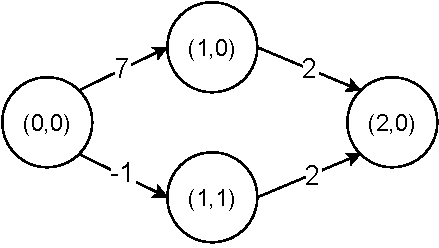
\includegraphics[width=0.4\textwidth]{Basic_Neural_Network.pdf}
%    \caption{A Simple Neural Network}
%    \label{Figure: Simple Neurla}
%
%\end{figure} 
%
%Figure \ref{Figure: Simple Neurla} depicts a feed forward neural network comprising four neurons: $n_0^{0}$, $n_0^{1}$, $n_1^{1}$, and $n_0^{2}$. The weight matrix between layer 0 and layer 1, denoted by $W_{0,1}$, is $[7, -1]^T$, and the bias matrix for layer 1, denoted by $B_{1}$, is $[0, 0]^T$. If we assign a value of 1 to the neuron $n_0^{0}$ (i.e., $v_0^{0}=1$), then the value of the neuron $n_0^{1}$ is $v_0^{1}=7$, as determined by $V_{1} = \phi([7, -1]^{T} \cdot [1] + [0, 0]^{T}) = [7, 0]^{T}$.
%
%
%\subsection{Neural Network Verification }
%In the context of neural network verification, we typically engage with a neural network, posing a ``$\textit{satisfiablility}$'' query to validate or refute a property. The query \(\mathcal{P}\) is structured as a triple, \(\mathcal{P} = \langle \mathcal{N}, \kappa, \lambda \rangle\). Here, \(\mathcal{N}\) denotes the neural network as previously mentioned, while \(\kappa\) and \(\lambda\) represent properties on the input and output neurons, respectively. 
%
%$\kappa$ is defined as a conjunction of linear constraints applied to the input neurons. Correspondingly, $\lambda$ is also expressed as a conjunction of linear constraints targeting the output neurons. Our objective is to verify boolean properties formulated as $\forall x \in X,\textit{ } y < c$. However, for the purpose of assessing the validity of these properties, we transform our $\lambda(y)$—the conjunction of constraints on our output variables—into the negation of $y < c$, represented as $y \geq c$, where $y$ denotes the output of the neural network. To achieve this transformation, we introduce additional neurons into the network, resulting in a modified network structure with a singular output neuron. This transformation of the Neural Network $\mathcal{N}$ proves advantageous for subsequent Inc/Dec classification, which is described in the subsequent section 2.3.1.
%
%Our query is constructed as a boolean formula \(\mathcal{P}(x) \equiv \kappa(x) \land \lambda(\mathcal{N}(x))\). Since we are looking for validity we use the negation of the output property and seek an `UNSAT'. The solver is presented with the formula \(\exists x \in X, \mathcal{P}(x)\), where \(X\) is the domain of the input. If our solver responds with `SAT' to this query, it indicates that we have identified a counterexample, and our property does not hold. Conversely, an `UNSAT' result signifies the validity of our original property.
%
%
%\subsection{Counter-example guided abstraction and refinement}
%To aid and expedite the verification queries, we employ a strategy to simplify our neural network by reducing the number of neurons. Our approach involves constructing an over-approximate network, denoted as $\mathcal{N''}$, where the output value, $\mathcal{N''}(x)$, consistently exceeds the value computed by the original network, $\mathcal{N}(x)$, i.e ($\forall x \in X, \hspace{1mm} \mathcal{N''}(x) \geq \mathcal{N}(x)$), where $X$ is our input domain. This simplification is undertaken because our property which is expressed as $\forall x \in X, \hspace{1mm} \mathcal{N}(x) < c$ can then be proven by determining the unsatisfiability of $\exists x \in X, \hspace{1mm}\mathcal{N''}(x) \geq c$. If the answer to this question is `Yes,' then it implies that $\forall x \in X, \hspace{1mm} \mathcal{N}(x) < c$ holds, as evidenced by ($\forall x \in X, \hspace{1mm} \mathcal{N''}(x) \geq \mathcal{N}(x)$).
%
%
%
%\subsubsection{Increment Decrement Splitting}
%To aid in the process of constructing such an over-approximate network we begin with the creation of an equivalent network, denoted as $\mathcal{N}'$, ensuring that $\mathcal{N'}(x)$ equals $\mathcal{N}(x)$ for all $x$. To build this equivalent network, we perform an `Increment/Decrement' splitting of neurons in our original network $\mathcal{N}$. Upon reflection, it became apparent to us that a two-class classification was more fitting for our needs, deviating from the initially recommended four-class classification outlined in the original work by \cite{b2}.
%Neurons are categorized as `Increment (Inc)' if increasing their values increases the output neuron's value, and as `Decrement (Dec)' if decreasing their values achieves the same result.
%
%\begin{algorithm}[H]
%    \caption{split\_Inc\_Dec}
%    \begin{algorithmic}[1]
%        \State Initialize M, the set of nodes that are marked, to \{out\_node\} and mark out\_node as \textbf{Inc}.
%        \State Let $R$ be the set of nodes with successors in $M$.
%        \State Define $\text{sign(u,v)}$ as the sign of the weight from the node $u$ to $v$.
%        \State Define $\text{Class(v)}$ as $1$ when $v$ is marked as $\textbf{Inc}$, and $-1$ otherwise.
%        \While {\text{node} $\notin M$ and node $\notin$ input\_nodes}
%        \State Pick a node $u$ such that $u \in R-M$
%        \State Suppose $u$ feeds into $x_1,x_2,x_3,..$ and $y_1,y_2,y_3..$ where $\text{sign($u,x_i$)} = \text{Class($x_i$)}$ for all $x_i$, $\text{sign($u,y_i$)} \neq \text{Class($y_i$)}$ for all $y_i$.
%        \State Split $u$ to $u_1$ and $u_2$, where $u_1$ feeds into all the $x_i$ and $u_2$ feeds into all the $y_i$.
%        \State Mark $u_1$ as \textbf{Inc} and $u_2$ as \textbf{Dec}
%        \State Insert $u_1$ and $u_2$ into $M$ and their predecessors into $R$
%        \EndWhile
%        \end{algorithmic}
%\end{algorithm}
%% \begin{algorithm}
%% \caption{splitIncDec}
%% \begin{algorithmic}[1]
%% \Require Graph $G$
%% \State $G.nodes[output\_node]['Inc/Dec']='Inc'$
%
%% \For{$layer$ in $reversed(G.intermediate\_layers)$}
%%     \For{$curr\_node$ in $layer$}        
%%         \For{$node$ in $G.adj[curr\_node]$}
%%             \State inc\_node, dec\_node are Inc/Dec copies of the curr\_node neuron
%%             \State $wgt = G.adj[node]['weight']$
%%             \If{$wgt > 0$ \textbf{and} $G.nodes[node]['inc/dec']=='inc'$}
%%                 \State $G.add\_edge(inc\_node, node, weight = wgt)$
%%             \ElsIf{$wgt < 0$ \textbf{and} $G.nodes[node]['inc/dec']=='dec'$}
%%                 \State $G.add\_edge(inc\_node, node, weight = wgt)$
%%             \ElsIf{$wgt < 0$ \textbf{and} $G.nodes[node]['inc/dec']=='inc'$}
%%                 \State $G.add\_edge(dec\_node, node, weight = wgt)$
%%             \ElsIf{$wgt > 0$ \textbf{and} $G.nodes[node]['inc/dec']=='dec'$}
%%                 \State $G.add\_edge(dec\_node, node, weight = wgt)$
%%             \EndIf
%%         \EndFor
%%     \EndFor
%% \EndFor
%% \end{algorithmic}
%% \end{algorithm}
%
%
%
%\subsubsection{Abstraction}
%
%\begin{figure}[H]
%    \centering
%    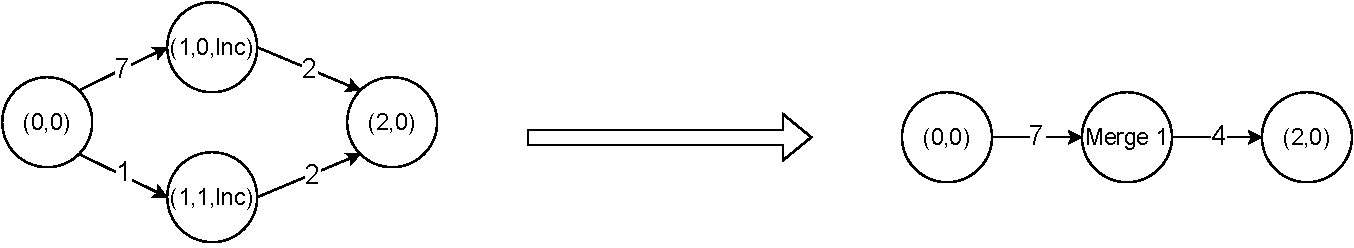
\includegraphics[width=0.9\textwidth]{Abstraction_part1.pdf}
%    \caption{Merging of Increment Neurons}
%    \label{Figure: Merge1}
%    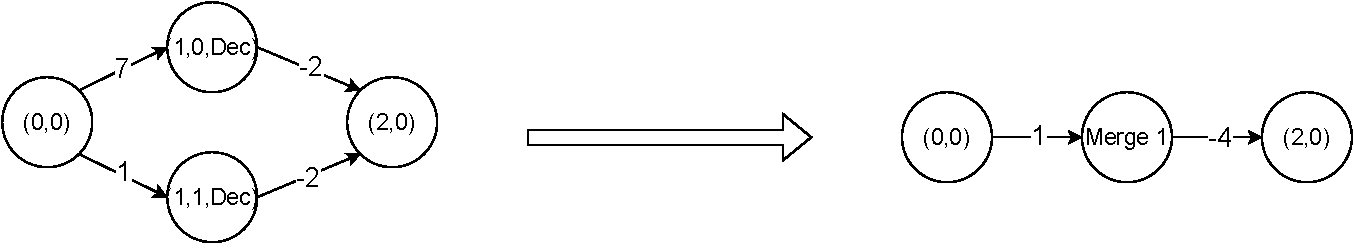
\includegraphics[width=0.9\textwidth]{Abstraction_part2.pdf}
%    \caption{Merging of Decrement Neurons}
%    \label{Figure: Merge2}
%
%\end{figure} 
%The increment/decrement splitting of the neural network $\mathcal{N}$ to the new network $\mathcal{N'}$ changes the structure of the neural network but does not change the value of the output neuron. If we want to construct a neural network $\mathcal{N}''$ which over-approximates the value of the original network $\mathcal{N}$ i.e $\forall x \in X, \hspace{1mm} \mathcal{N''}(x) \geq \mathcal{N}(x)$, then we perform the following steps:
%\begin{enumerate}
%    \item When merging two $\textit{Increment Neurons}$, discard one of those neurons and replace the incoming weight by maximum of all the incoming weights and the outgoing weight by summation of all the outgoing weights. 
%    \item When merging two $\textit{Decrement Neurons}$, discard one of those neurons and replace the incoming weight by minimum of all the incoming weights and the outgoing weight by summation of all the outgoing weights. 
%\end{enumerate}
%
%
%\subsection{Refinement }
%After merging the neurons, we introduce an over-approximation into the new network $\mathcal{N''}$. And since $\mathcal{N''}(x) \geq \mathcal{N}(x)$, there might exist a $x$, for which, $\exists x \in X, \hspace{1mm} \mathcal{N''}(x) \geq c$ but $\nexists x \in X, \hspace{1mm} \mathcal{N}(x) \geq c$. Therefore, if a counter-example `$\beta$' returned is not a valid counter-example, which means, $\mathcal{N''}(\beta) \geq c > \mathcal{N}(\beta)$, then, we must reverse some of the merges performed previously to get a new network which mitigates the extent of the over-approximation for us to get a valid counter-example or to prove that the original property is valid.
%
%In \cite{b2}, the authors employed a Counterexample-Guided Abstraction Refinement (CEGAR) approach to eliminate the spurious counter-examples. They utilized a counter-example ($\beta$) to identify a neuron $n_i^j$ that had been merged into the node `$r$' for refinement. The authors then computed the value $\omega$ which was equal to $|v_i^j(\beta) - r(\beta)| \cdot |w_{n_{i-1,k},n_{i,j}}-w_{n_{i-1,k},r}|$, where $v_i^j(\beta)$ denotes the value of $n_{i,j}$ at the counter-example $\beta$, $r(\beta)$ denotes the value of the representative neuron $r$ at the counter-example $\beta$, $w_{n_{i-1,k},n_{i,j}}$ denotes the weight between a neuron $n_{i-1,k}$ and a neuron $n_{i,j}$. If this value $\omega$ was over a recommended amount $\epsilon$, they proceeded to separate $n_i^j$ from $r$ to potentially eliminate the spurious counter-example $\beta$.
%
%
% In the next section, we present a new method for merging neurons in order to reduce the number of refinement steps, thereby expediting the verification process.
%
%\section{Methodology}
%
%Our methodology involves two broad steps:
%\begin{enumerate}
%    \item Finding a tree structure that represents the order in which neurons should be merged.
%    \item Using that structure to guide a CEGAR approach in order to help reduce number of refinement steps.
%\end{enumerate} 
%
%\subsection{Tree and Merges:}
%
%To establish the merging order of neurons, we create a tree structure wherein leaf nodes represent the original neurons, and non-leaf nodes represent merge groups. The construction of the tree follows a bottom-up approach, prioritizing the merging of similar neurons and delaying the merging of dissimilar ones. Similarity is ascertained through observation vectors. Consider simulating the network with distinct input values and observing the fluctuating values of a particular neuron corresponding to those inputs. The collection of these observed values constitutes an observation vector. 
%
%\begin{figure}[H]
%    \centering
%    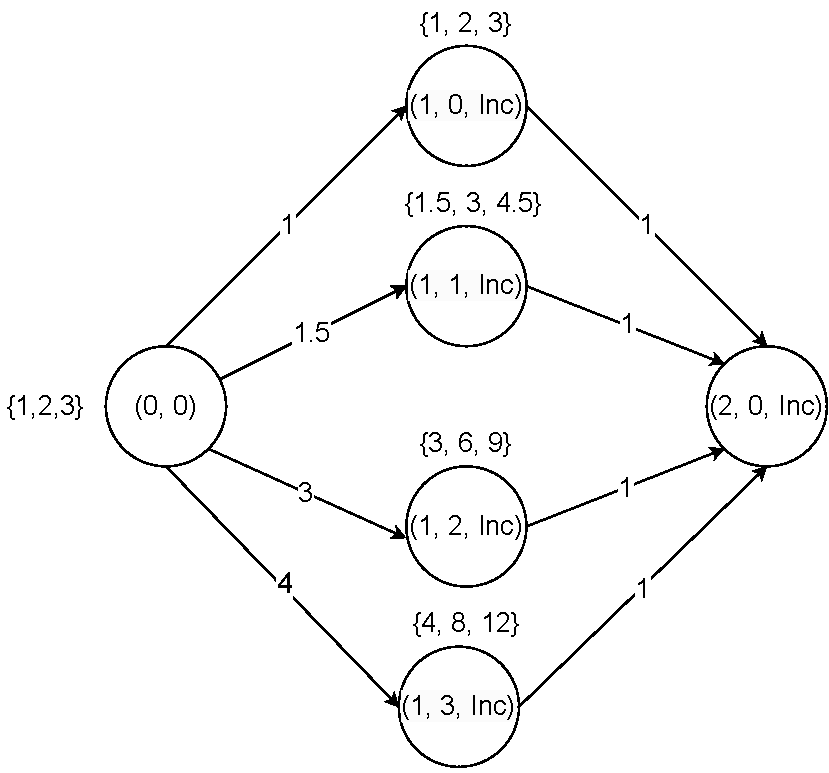
\includegraphics[width=0.5\textwidth]{tree_merges.pdf}
%    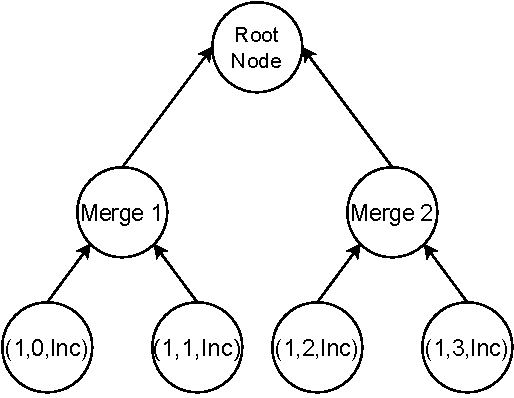
\includegraphics[ width=0.47\textwidth]{Order_of_Merge.pdf}
%    \caption{Order Of Merging}
%    \label{Figure: Order Of Merging}
%\end{figure}
%
%
%In Figure \ref{Figure: Order Of Merging}, when we input values \{1, 2, 3\} to the neuron $n_0^{0}$ at different time instances, we obtain corresponding values \{1.5, 3, 4.5\}, forming the observation vector at neuron $(n_1^{1},Inc)$. For instance, considering three neurons $n_i^{w}$, $n_j^{w}$, and $n_k^{w}$ with observation vectors $\mathcal{\nu}(n_i^{w})$, $\mathcal{\nu}(n_j^{w})$, and $\mathcal{\nu}(n_k^{w})$, the merging sequence adheres to the following conditions: 
%
%If $||\mathcal{\nu}(n_i^{w}) - \nu(n_j^{w})||_{2} \leq ||\nu(n_i^{w}) - \nu(n_k^{w})||_{2}$ and $||\nu(n_i^{w}) - \nu(n_j^{w})||_2 \leq ||\nu(n_j^{w}) - \nu(n_k^{w})||_{2}$, then $n_i^{w}$ and $n_j^{w}$ are initially merged into a representative neuron $\alpha$, followed by the merging of $\alpha$ and $n_k$. Here $||\nu(n_i^{w}) - \nu(n_j^{w})||_{2}$ computes the ``$\textit{Euclidean  Distance}$" between the observation vectors $\nu(n_i^{w})$ and  $\nu(n_j^{w})$.
%
%
%In Figure \ref{Figure: Order Of Merging}, for the first layer, the initial merge would involve the neuron $(n_0^{1},Inc)$ with $(n_1^{1},Inc)$, forming $\textit{Merge 1}$, then we would combine $(n_2^{1},Inc)$ and $(n_3^{1},Inc)$, forming $\textit{Merge 2}$. Finally we combine $\textit{Merge 1}$ and $\textit{Merge 2}$ into the root node. 
%
%As we progress up the tree, the degree of over-approximation rises. This is due to the increasing difference between observation vectors as we ascend. Therefore, the sub-trees closer to the root are indicative of coarser merges, whereas the ones farther from the root represent finer merges. 
%
%
%
%\subsection{Using Counter-Examples to make cuts in the Tree} 
%We are guided by this tree as a prospective refinement method. Starting with the entire tree where everything is merged. When the solver detects a spurious counterexample `$\beta$', we leverage it to refine the network. This process commences by identifying the ``culprit neuron $\gamma$'' selected for refinement. A ``culprit neuron'' in a merge group is selected on the basis of how much the neuron contributed to the output. If change in output of  neuron changes the value of the output neuron significantly then that neuron is a good candidate for ``culprit neuron". 
%
%Following this, we reverse all merges dependent on the culprit neuron $\gamma$. Therefore, refinement essentially involves finding a cut-point in the tree, precisely where all merges dependent on the culprit neuron $\gamma$ are undone. Each cut produces a set of trees, the merge groups then consist of neurons in the leaf nodes of the  these trees. Therefore finding new merge groups for refinement is therefore just finding a cuts in the tree.
%
%\begin{figure}
%    \centering
%    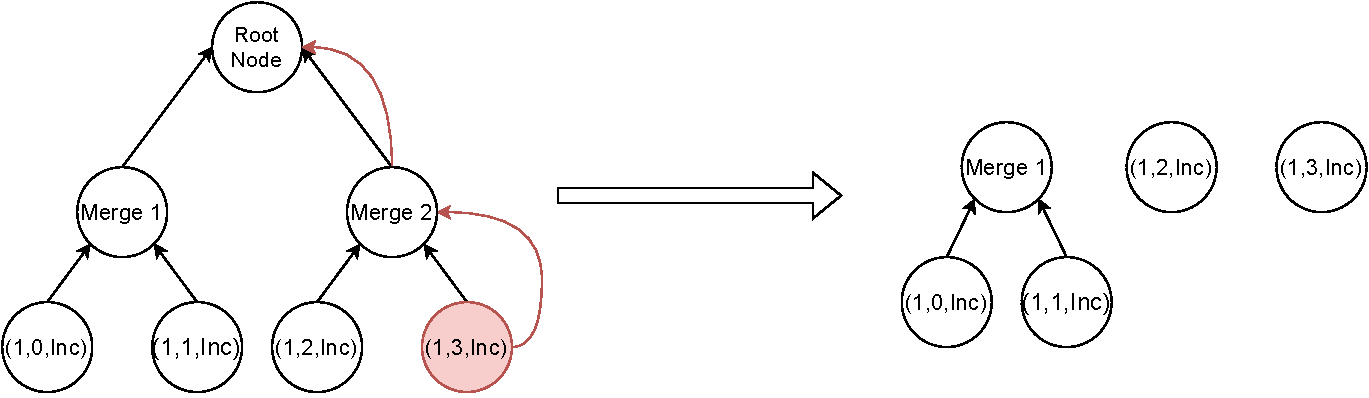
\includegraphics[width = 0.9\textwidth]{_before and after cut.pdf }
%    \caption{Trees and Cuts}
%    \label{Figure 2}
%\end{figure}
%
%Consider Figure \ref{Figure 2}, illustrating the merging sequence of neurons $(n_0^{1}, Inc)$, $(n_1^{1}, Inc)$, $(n_2^{1}, Inc)$, and $(n_3^{1}, Inc)$. If, for instance, the neuron $(n_3^{1}, Inc)$ is identified as the problematic neuron based on a counter-example, we will reverse all the merges dependent on the $(n_3^{1}, Inc)$ neuron, including $\textit{Merge 2}$ and the $\textit{Root Node}$ merge. Consequently, after implementing this reversal indicated in Figure \ref{Figure 2}, our refinement phase will yield three distinct merge groups. The first merge group comprises two neurons, namely $(n_0^1, Inc)$ and $(n_1^1, Inc)$. The second merge group and the third merge have single neurons $(n_2^1, Inc)$ and $(n_3^1, Inc)$, respectively.
%
%\subsection{Culprit Neurons} 
%
%A neuron, denoted as $\gamma$, is designated as a culprit neuron within a specific layer when absolute value of the product of the difference between $(v_{Rep(\gamma)}$ and $v_{\gamma})$ and the effective weight is maximized.
%
%
%$||(v_{Rep(\gamma)} - v_{\gamma})||_{2} \cdot |(\textit{effective\_weight})|$
%
%In this context, $Rep$ signifies the representative neuron for neuron $\gamma$, $v_{\gamma}$ represents the value of the neuron $\gamma$ at counter-example $\beta$ and $\textit{effective\_weight}$ represents the how much does the value of output neuron changes with respect to change in the value of the neuron under consideration, essentially corresponding to the ``$\textit{gradient}$'' at that particular counter-example ``$\beta$''.
%
%\begin{algorithm}
%    \caption{Finding Cuts in the Tree (find\_new\_merge\_groups)}
%    \begin{algorithmic}[1]
%        \State $\gamma= \arg \max_i \|v_{Rep(i)} -v_i \|_2 \cdot | \textit{effective\_weight}| $ 
%        \State Find a sequence of nodes, $t_1,t_2,t_3,..,t_k$ representing a  path from $t_1=$root to $t_k=\gamma$.
%        \State Remove the nodes $t_1,t_2,..,t_{k-1}$ denoting the merges dependent on $\gamma$ through this path, leading to our connected tree being split into a collection of disconnected sub-trees.
%        \State New merge groups are the leaf nodes in our disconnected graph.
%    \end{algorithmic}
%    \hspace*{\algorithmicindent} \textbf{Output} New Merge Groups
%\end{algorithm}
%
%\subsection{Optimality of the Trees}
%Our objective is to determine the most efficient order for merging neurons, minimizing the introduction of over-approximation at each step. This approach aims to avoid creating networks with excessive over-approximation, which could lead to the generation of spurious counter-examples in response to queries. Opting not to mitigate over-approximation at each step would result in an increased number of refinement steps. This essentially entails making additional solver calls, incurring significant costs to eliminate the spurious counter-examples.
%
%
%Nevertheless, during the initial merging process (until saturation is reached), the root node ``$\rho$'' will exhibit the same level of over-approximation across all conceivable merging scenarios—for all possible tree sequences. Nevertheless, when we descend one level down the tree to explore the children nodes of our original root node $\rho$ for the purpose of identifying a cut for refinement, we discover varying levels of over-approximation manifesting in the root nodes of the resultant sub-trees. These differences are a result of the different merging scenarios pursued to construct those individual trees.
%
%\begin{algorithm}[H]
%\caption{Cluster Merging Algorithm (find\_abstraction\_tree)}
%\label{Cluster Merging Algorithm}
%\begin{algorithmic}[1]
%    \State Initialize every simulated distance vector as a singleton cluster.
%    \State Initialize $C=\{v_1,v_2,v_3,..\}$ as the set of singleton clusters.
%    \State Initialize a Binary Tree $T$ with leaves as $\{(n_1),(n_2),(n_3),..\}$ corresponding to $\{v_1,v_2,v_3,..\}$.
%    \State Initialize $V$ as a set of visited nodes, empty at first.
%    
%    \Function{MergeFunction}{$u, v$}
%        \If{All nodes are classified as \textbf{Inc}}
%        {
%        
%            \Return $\max(u, v)$
%        }
%        \Else{ }
%        {
%        
%            \Return $\min(u, v)$
%        }
%        \EndIf
%    \EndFunction
%    
%    \While{$|C|>1$}
%        \State $v_j, v_j = \arg\min_{\substack{a, b \in C}} \| a - b \|_2$
%        \State Set $w=\text{MergeFunction}(v_i,v_j)$
%        \State Let nodes from $T$ not in $V$ corresponding to $v_i,v_j$ be $m_i$ and $m_j$
%        \State Remove $v_i,v_j$ from $C$ and add $w$ to $C$.
%        \State Make $(m_i \cup m_j)$ the parent of $(m_i)$ and $(m_j)$ in tree $T$
%        \State Add $m_i$ and $m_j$ to $V$.
%    \EndWhile
%\end{algorithmic}
%\end{algorithm}
%
%While the optimal tree, representing the optimal merging sequence, can aid in the refinement process by guiding the reversal of merges, finding such an optimal tree poses is extremely challenging. Even when dealing with only `n' Increment (Inc) neurons that have been merged to saturation, the total number of possible trees is given by $(2n-3)!!$, making the task of determining the truly optimal tree from these options extremely challenging.
%
%Since finding this ideal tree is a challenging task, we employ hierarchical clustering (Algorithm \ref{Cluster Merging Algorithm}) as an approach to approximate and derive such a tree. Initially, we simulate our network using a set of `$k$' inputs. Subsequently, we employ cluster analysis on these `$k$' points to construct a hierarchical arrangement of clusters. This process initiates with data points corresponding to simulated values (observation values in the observation vector) of a neuron  forming their own cluster. The clusters are then systematically combined based on their similarity, thereby generating a hierarchy of clusters. The choice of similarity measure is the ``$distance \hspace{1mm} metric$" between clusters. We have used ``$Euclidean \hspace{1mm} Distance$" as our distance metric. Given that the data points to perform this hierarchical clustering originate from the values of the simulated neurons, this hierarchical clustering effectively reflects the methodology we employ to merge the neurons.
%
%For example, in Figure \ref{Figure: Order Of Merging}, we conducted a simulation of our network on three data points. Subsequently, we examined the observation vectors corresponding to these points. Utilizing the hierarchical clustering algorithm, the initial selection for merging  will involve $(n_0^{1}, Inc)$ and $(n_1^{1}, Inc)$ because of the fact that their Euclidean distance is minimum. This forms $\textit{Merge 1}$ in Figure \ref{Figure: Order Of Merging}. The observation vector for $\textit{Merge 1}$ ($\nu_\textit{Merge1 }$) is the max of the $\nu((n_0^{1}, Inc))$ and $\nu((n_1^{1},Inc))$ which is \{1.5, 3, 4.5\}. For decrement nodes the observation vector would be minimum of the observation vector of the corresponding decrement nodes. The next merging step involved selecting $\nu((n_2^{1}, Inc))$ and $\nu((n_3^{1}, Inc))$ and merging these two neurons, representing $\textit{Merge 2}$ in Figure \ref{Figure: Order Of Merging}. The observation vector for $\textit{Merge 2}$ is now \{4, 8, 12\}. Ultimately, the Merge1 merge group is merged with the $\textit{Merge 2}$ merge group to create the Root Node in our network.
%
%\begin{figure}[H]
%    \centering
%    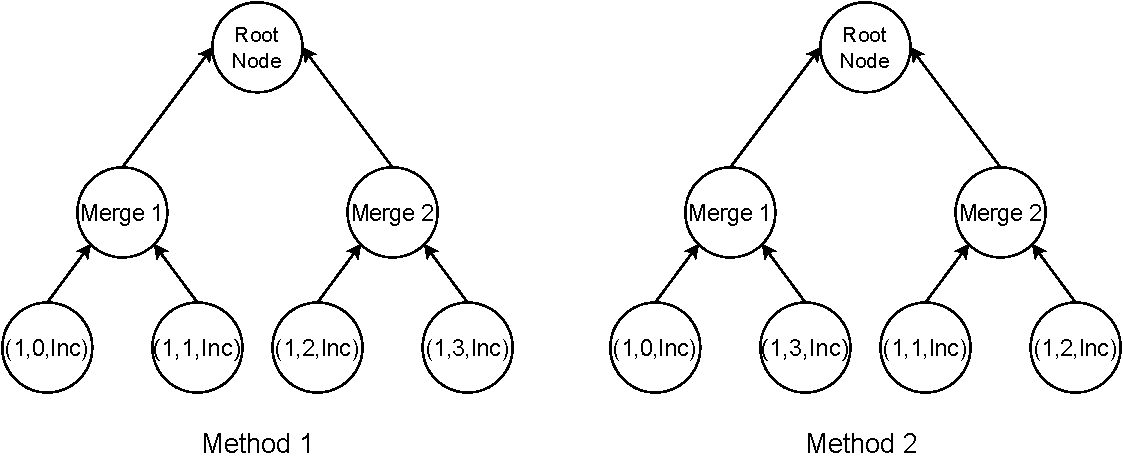
\includegraphics[width = 0.9\textwidth]{good_vs_bad_merges.pdf}
%    \caption{Ways of Merging}
%    \label{Figure 3}
%\end{figure}
%
%This approach of merging neurons based on similarity proves advantageous as it helps in reducing number of refinement steps. For instance, consider the task of checking whether $\forall v_{0}^{0} \in [0, 1]$ implies $v_{0}^{2} < 10$. If we had the neuron $(n_{3}^{1}, Inc)$ as the culprit neuron and then if we follow the second merging approach depicted in Figure \ref{Figure 3}, then we would have been compelled to reverse both $\textit{Merge 1}$ and $\textit{Merge 2}$. However, by employing the first merging approach, undoing only the $\textit{Merge 2}$ becomes sufficient, resulting in a reduction in the number of refinement steps required.
%
%
%\subsection{Overall Algorithm}
%\begin{algorithm}[H]
%    \caption{Overall Algorithm}
%    \label{Overall Algorithm}
%    \begin{algorithmic}[1]
%        \State $\mathcal{N'}$ = split\_Inc\_Dec($\mathcal{N}$)
%        \State $\mathcal{N''}$ = abstract\_network($\mathcal{N'}$)
%        \State simulation\_dict = simulate\_network($\mathcal{N'}$)
%        \State $\mathcal{T}$ = find\_abstraction\_tree($\mathcal{N'}$, $simulation\_dict$)
%        \If{verify($\mathcal{N''}$, $\kappa$, $\lambda$) is UNSAT}{
%
%            \Return Property Holds
%            }
%        \Else
%            \State Extract counter-example $\beta$
%            \If{$\beta$ is not a spurious counter-example}
%            {
%
%                \Return ($\beta$, Property Violated)
%            }
%            \Else
%                \State Find culprit neuron $\gamma$
%                \State $merge\_groups$ = find\_new\_merge\_groups($\mathcal{T, \gamma}$)
%                \State $\mathcal{N''} = get\_abstract\_network(merge\_groups)$
%                \State \textbf{goto} step 5
%            \EndIf
%        \EndIf
%    \end{algorithmic}
%\end{algorithm}


\section{Experiments} 

We have implemented our method in python\footnote{The entirety of the code,
networks, datasets, and properties utilized in our evaluation will be made
available via a publicly hosted code repository in the camera ready version.}, 
utilizing the NumPy library for linear algebra
operations and the SciPy library for an implementation of \hcluster.
We have used a linkage-matrix based data structure similar to the one used in
SciPy to store the tree, and have precomputed and cached several
operations that may need to be repeated every refinement iteration. This allows
us to quickly perform the merge and split operations and calculate the
scores (Section \ref{s:refinement}), without having to do (relatively)
expensive tree traversal operations in each iteration of the abstraction
refinement loop. 

Using this implementation, we have performed a set of experiments demonstrating
the effectiveness of our abstraction technique for verification of neural
network queries on the \acasxu set of networks, using both the original safety
properties from \cite{reluplex} and the $\epsilon$-robustness properties
introduced in \cite{cegar-nn}. To do so, we set up a \cegar loop (Section
\ref{s:abs-ref-fw}) using our abstraction technique, using the \neuralsat solver
as the underlying solver to dispatch the verification queries on \abs.
We compare our abstraction framework with the existing \cegar framework proposed
in \cite{cegar-nn} \footnote{We have used a faithful re-implementation of this
framework that follows exactly the procedure in the paper, with the only two
distinctions being that we are using a two-class classification as seen in
\cite{chauhan2022efficiently,liu2022abstraction,10.1145/3644387},
and that the call to verify the \abs obtained in each iteration is sent to an
instance of the \neuralsat solver as opposed to \marabou. } 
setting a 
timeout of 200 seconds for each instance in the benchmark and for both the
our technique and the existing work.
The experiments were run on a machine running on Intel(R) Core(TM) 
i7-6700 CPU with 8 CPUs running at 3.40GHz, having 16 GB RAM and running running 
Ubuntu 22.04 LTS.

If the \abs produced has multiple neurons with the exact same set of incoming
edges in the same layer, these neurons compute the same function and are
redundant. Therefore, as an added optimization step in our method, 
\dmcmt{This is regd comment from review 2, saying its not clear if this is done
    for guy katz's method as well. It was not. Is it okay to just say this, or
do we need to be more explicit?}
we safely \textit{re-merge}
them by taking the sum of the outgoing edges. Note that this does not change the
behavior of \abs.

%to
%demonstrate the usefulness of our technique. To begin with, we demonstrate 
%the application of our method within a CEGAR loop, as outlined in \cite{cegar-nn}, 
%for verifying the \acasxu properties (refer to Section \ref{s:acas-verif}). 
%In these experiments, we employed \neuralsat as the solver in the backend.
%In our subsequent experiments, we illustrate the utility of our abstraction 
%technique in achieving efficient compression of \dnn within safety-critical 
%environments. We ensure that this compression doesn't introduce any new 
%false negative classifications, as detailed in Section \ref{s:exp-mnist-comp}. 
%This necessity is crucial, especially in scenarios such as medical diagnosis 
%and collision detection, where the application of \dnn as classifiers necessitates 
%precise measures to prevent false negative classifications for specific classes.
%Finally, we demonstrate how our technique may be used to obtain abstract 
%networks with the aim of proving a given property, plotting the number of 
%spurious counterexamples introduced as the size of the abstract network 
%reduces (Section \ref{s:exp-mnist-rob}). 

%If the \abs produced has multiple neurons with the exact same set of incoming
%edges in the same layer, these neurons compute the same function and are
%redundant. Therefore, as an added optimization step, we safely \textit{re-merge}
%them by taking the sum of the outgoing edges. Note that this does not change the
%behavior of \abs.

%The experimental results in Tables \ref{t:acas-verif}, \ref{t:acas-verif-robustness} and Figure
%\ref{f:scatter-netsizes} were produced on a machine running on Intel(R) Core(TM) 
%i7-6700 CPU with 8 CPUs running at 3.40GHz, having 16 GB RAM and running running 
%Ubuntu 22.04 LTS. The results in Tables \ref{t:mnist-compr-summary}, \ref{t:acas-ncex}
%and Figures \ref{f:mnist-class}, \ref{f:acas-ncex-samples} were run on a 
%machine running on an Intel(R) Core(TM) i7-9700K with 8 CPUs running at
%3.60GHz, having 16 GB RAM and running Ubuntu 22.04 LTS. 
%The results in Figures \ref{f:mnist-prop-samples} and Table \ref{t:mnist-prop-summary} were produced on a 
%machine running on an Intel(R) Core(TM) i7-13700 with 24 CPUs running at
%5.20GHz, having 32 GB RAM and running Ubuntu 23.10.

%\subsection{Verification of \acasxu}
%\label{s:acas-verif}

%In this set of experiments, we demonstrate the effectiveness of our abstraction
%technique for verification of neural network queries on the \acasxu set of
%benchmarks. To do so, we set up a \cegar loop (Section \ref{s:abs-ref-fw}) using
%our abstraction technique, where on each \abs generated we call \neuralsat. 
%If the solver returns a spurious counterexample, we use
%that as $\vct{\beta}$ to refine our network according to Section
%\ref{s:refinement}.  

%For these experiments, we have used \neuralsat as the solver. 
%We compare our abstraction framework with an existing \cegar framework proposed
%in \cite{cegar-nn} \footnote{We have used a faithful re-implementation of this framework that
%follows exactly the procedure in the paper, with the only distinction being that
%the call to verify the \abs obtained in each iteration is sent to an instance of
%the \neuralsat solver as opposed to \marabou. \dmcmt{Is this okay?}}. We set a
%timeout of 200 seconds for each instance in the benchmark and for both the
%our technique and the existing work \cite{cegar-nn}.

\begin{table}
    \vspace*{-0.25cm}
    \centering
        \begin{tabular}{ |c|c|c|c|c| }
        \hline
        Method                   & No. Safe    & No. Unsafe & No. Timeout & Average Size \\ 
        \hline
        Ours                     &   121       & 43         & 16          &  335.3\\
        Existing \cite{cegar-nn} &   118       & 43         & 19          &  536.0\\
        \hline                                                                
        \end{tabular}
        \caption{Summary of \acasxu on original safety properties }
        \label{t:acas-verif}
    \vspace{-1.5cm}
\end{table}
\begin{table}
    \centering
    \begin{tabular}{ |c|c|c| }
    \hline
    Method                   & Percentage Verified  & Average Size \\ 
    \hline
    Ours                     &   100\%              &  27.9\\
    Existing \cite{cegar-nn} &   100\%              &  31.5\\
    \hline                                                                
    \end{tabular}
    \caption{Summary of \acasxu on robustness properties }
    \label{t:acas-verif-robustness}
    %\vspace{-1cm}
    \vspace*{-0.75cm}
\end{table}


Tables \ref{t:acas-verif} and \label{t:acas-verif-robustness} summarizes the
results on these benchmarks. We
find that using our framework, we are able to perform better than the existing
\cegar approach \cite{cegar-nn} on the original safety properties, verifying
more networks to be safe, while we do not loose performance on the robustness
properties. 

\begin{wrapfigure}{r}{0.5\textwidth}
    \vspace*{-0.5cm}
    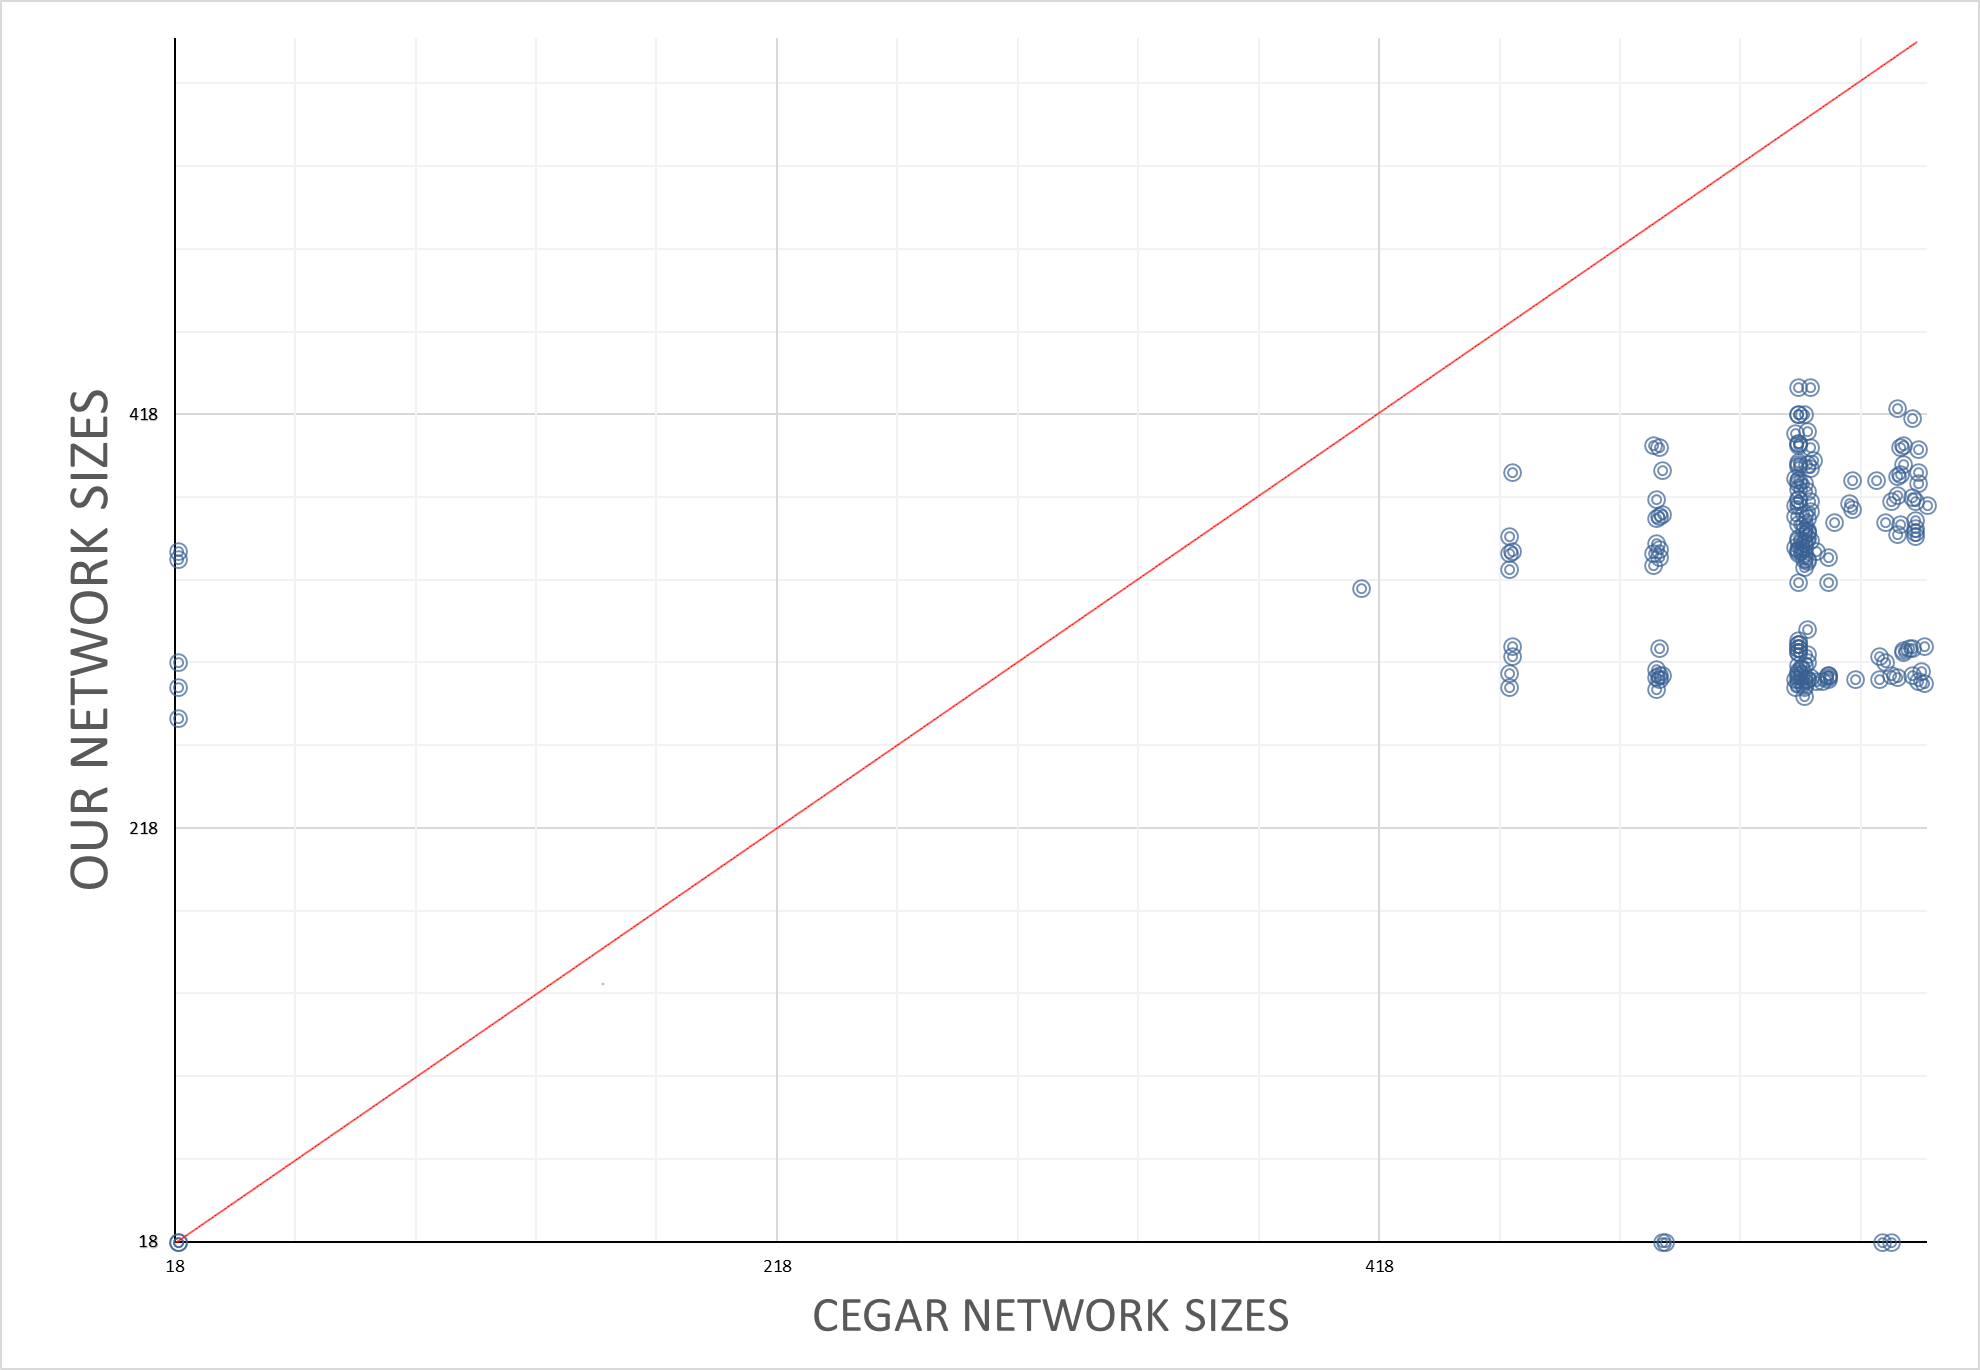
\includegraphics[scale=0.2]{figs/scatter-cegar-our-nerualsat-diag.png}
    \caption{Scatter plot of network sizes produced by our framework vs existing
    work \cite{cegar-nn} on \acasxu \todo{Make label bigger on graph}}
    \label{f:scatter-netsizes}
    \vspace*{-0.5cm}
\end{wrapfigure}

For each framework, we collected the final \abs at the end of the \cegar
iterations, for which either the property can be proved to be safe, or 
the solver is able to find an actual counterexample, or the solver times out.  
Figure \ref{f:scatter-netsizes} shows a scatter plot comparing the sizes of
these final \abs obtained by our framework and by existing work \cite{cegar-nn}
for each instance in the benchmark.
A point below the red diagonal line represents an instance for which we obtain a
smaller final \abs than the existing work, therefore points below the line
represent instances for which we perform better.
The average sizes of these \abs over all instances are
reported in the `Average Size' columns in tables \ref{t:acas-verif} and
\label{t:acas-verif-robustness}. 

It is apparent from the Figure \ref{f:scatter-netsizes}, 
table \ref{t:acas-verif} and table \ref{t:acas-verif-robustness} that compared 
to the existing techniques, we are explore smaller \abs that are effective 
at proving or disproving the property in question.
This shows that using semantic information to guide the CEGAR process can
effectively find more efficient abstractions than the existing technique.

Note that in our experiments, we found that the time taken by both our CEGAR
approach and the existing CEGAR approach \cite{cegar-nn} was more than what the
\neuralsat solver takes for the \acasxu benchmarks. However, while we would
expect the solver call times to exponentially scale with network size, the
overheads from the abstraction procedure will not scale exponentially. Thus, for
larger and larger benchmarks, being able to find smaller \abs will produce a
significant difference in times. Furthermore, we believe that a verified \abs is
useful beyond verifying a single property - it may be used for other related
queries, or may be useful as a safely deployable compressed network.

Additionally, we find that the final solver times on the \abs are actually
comparable with the times obtained on the original un-abstracted \cnc. In
general it has may observed, both by our experiments and in \cite{cegar-nn},
that the effort needed to verify a network is dependent
on more than just network size. In fact, in \cite{cegar-nn},
they are able to achieve smaller solver times on larger networks. 
While it is true that in general the worst-case performance of neural network
solvers will almost certainly remain exponential in the size of the network
\cite{reluplex}, other factors on which the performance of neural network
solvers may depend on remains an interesting direction of future work. 



\printbibliography
    
\end{document}
 

